\newpage
\section{\label{migr}migr / migr\_mpi}

\subsection{General}
Shot record migration scheme based on optimized x-w wave field extrapolation operators. 

There is also a parallel version of {\tt migr} called {\tt migr\_mpi}. The parallelisation is based on MPI and the number of shot gathers to be migrated is divided over the number of available working processors. For reading the shot records the master processors reads all the shots and sent the data to the working processors. If a working processor has finished its migration the image (and eventually extrapolated source and receiver wavefields) are communicated back to the master processor, who will write the data to output file(s). 

\subsection{Parameters}
Via the command-line or in a parameter file: {\tt par=$<$parameter\_file$>$}.
{\footnotesize
\begin{verbatim}
 MIGR - pre-stack depth migration (x-w).
  
 migr file_shot= file_vel= [optional parameters]
  
 Required parameters:
 
   file_shot= ............... input data to be migrated
   file_vel= ................ gridded velocity file for receiver field
   file_vels=file_vel ....... gridded velocity file for source field
  
 Optional parameters:
 
   conjg=0 .................. 1: take complex conjugate of input data
   key=sx ................... input data sorting key for receiver field
   nxmax=512 ................ maximum number of traces in input file
   ntmax=1024 ............... maximum number of samples/trace in input file
 MIGRATION 
   imc=1 .................... image condition (*)
   ndepth=all ............... number of depth steps
   zrcv=oz .................. receiver depth level
   ixa=tan(alpha)*ndepth*dz . number of traces after acquisition aperture
   ixb=ixa .................. number of traces before acquisition aperture
   ntap=0 ................... number of taper points at boundaries
   eps_a=0.0 ................ absolute stabilization factor for imc=[1,2]
   eps_r=0.001 .............. relative stabilization factor for imc=[1,2]
   domain=1 ................. 1: x-w lateral variant convolution, 0: kx-w
   zomigr=0 ................. 1: zero-offset migration (=> velocity *= 0.5)
            ................. 2: zero-offset migration (=> velocity *= 1.0)
 SOURCE DEFINITION 
   file_src=<file_name> ..... (areal)wavelet used 
   key_src=fldr ............. input data sorting key for source field
   fmin=0 ................... minimum frequency 
   fmax=70 .................. maximum frequency
   conjgs=0 ................. 1: take complex conjugate of source wavefield
   selev=0 .................. 0: ignore headers for source/receiver depth
 EXTRAPOLATION OPERATOR DEFINITION 
   select=10 ................ type of x-w operator (*)
   opl=25 ................... length of the convolution operator (odd)
   alpha=65 ................. maximum angle of interest
   perc=0.15 ................ smoothness of filter edge
   weight=5e-5 .............. weight factor in WLSQ operator calculation
   beta=3 ................... 2 < beta < 10; factor for KAISER window
   fine=10 .................. fine sampling in operator table
   filter=1 ................. apply kx-w filter to desired operator
   limit=1.0002.............. maximum amplitude in best operators
   opl_min=15 ............... minimum length of convolution operator
 OUTPUT DEFINITION 
   file_image= .............. output file with migrated result
   writeafter=10 ............ writes image/shots after # processed shots
   file_ishot=NULL .......... output file for migrated shot-records
   writeshots=0 ............. 1; writes migrated shot record
   writeinc=1 ............... trace increment of file_ishots
   verbose=0 ................ =1: shows various parameters and results
   sx_file= ................. file with extrapolated source field
   rx_file= ................. file with extrapolated receivers
   depthex= ................. depth to save extrapolated fields (m)
  
   Options for select:
         - 0 = Truncated operator
         - 1 = Gaussian tapered operator
         - 2 = Kaiser tapered operator
         - 3 = Smoothed Phase operator
         - 4 = Weighted Least Squares operator
         - 5 = Remez exchange operator
         - 8 = Smooth Weighted Least Squares operator (careful if dz<0.5*dx)
         - 9 = Optimum Smooth Weighted Least Squares operator
         - 10= Optimum Weighted Least Squares operator (Default)
   Imaging condition:
         - 0 = correlation
         - 1 = stabilized inversion
         - 2 = stabilized Least Squares
         - 4 = 2*data.r for zero-offset migration only
         - 5 = smoothed imaging P265 EAGE 2006: A. Guitton
 
  The shot and receiver positions in the model are determined by
  the hdr values gx and sx. The data from file_shot is extrapolated 
  backward, the data from file_src is extrapolated forward.
  If file_src is not set a spike is taken, if file_src=pipe read from stdin
  Note that with the conjg and conjgs options the extrapolation 
  direction can be changed.
 
  Copyright 1997, 2008 Jan Thorbecke, (janth@xs4all.nl) 

\end{verbatim}}

\subsection{General parameter description}

The shots to be migrated ({\tt file\_shot}) and the gridded subsurface files ({\tt file\_vel} and {\tt file\_vels}) should have the same lateral extend being defined by the {\tt gx} headers.  The position of the receivers of the data in the subsurface grid is done by means of the {\tt gx} header value of the velocity model corresponding to the {\tt gx} header value in the data to be extrapolated. The distance between the traces in the velocity model should be smaller or equal to the distance between the receivers/shots. The program assigns the {\tt gx} value of the receivers to the nearest grid point in the velocity model. The number of depth steps is controlled with the parameter {\tt ndepth=}. To avoid reflections at the edges of the model the parameter {\tt ntap} can be set. {\tt ntap} indicates the number of points at the edges for which a spatial taper is designed according to: $\exp{(-(0.4*(ntap-ix)/ntap)^2)}$. Choosing {\tt ntap} equal to half of the operator length is an optimimum value. 
 
Topography is taken into account by using a velocity model which has zero velocities above the defined topography. In that case the position of the source and receivers is lowered into the velocity model until a non-zero velocity is found. From that depth the extrapolation of that point is started. 

The parameter {\tt file\_src} describes the source wavelet. If {\tt file\_src} is not defined a band-limited spike is assumed. If {\tt file\_src} contains only one trace it is assumed that this trace is the wavelet used for all shots to be migrated. If {\tt file\_src} contains more than one trace it is interpreted as an areal shot record and areal short-record migration is carried out. 

The parameters {\tt ixa} and {\tt ixb} determine the number of traces to be included in the calculation of a image gather. 
{\tt ixa} defines the number of traces to include in the calculation with a lateral position greater than the lateral extend (max value of {\tt sx,gx}) of the shot gather ({\tt a} from after). 
{\tt ixb} defines the number of traces to include in the calculation with a lateral shot position smaller than the lateral extend (max value of {\tt sx,gx}) of the shot gather ({\tt b} from before).


For a more detailed discussion on the different parameters which are related to the extrapolation operator optimization the reader is referred to the description of the program \htmlref{{\bf opercalc}}{opercalc}. The WLSQ operators are described in Thorbecke et al. (2004).

\subsection{Examples}

Generating a pulse repsonse through the medium of Figure \ref{model}. 

{\footnotesize
\begin{verbatim}
migr file_shot=ricker_shift.su file_vel=syncline_cp.su zomigr=1 file_image=migr8.su verbose=1 ixa=301 select=8
suximage < migr8.su 
migr file_shot=ricker_shift.su file_vel=syncline_cp.su zomigr=1 file_image=migr10.su verbose=1 ixa=301 select=10
suximage < migr10.su 
\end{verbatim}}

%
\begin{figure}[hb]
  \begin{pspicture}(8,4.2)
    \put(-0.5,-0.3){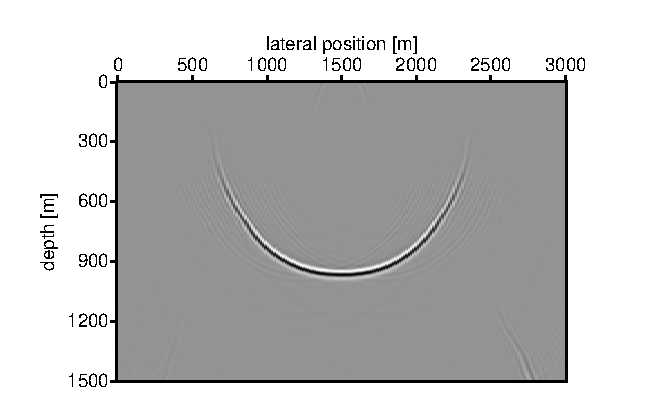
\epsfig{file=EPS/migr_puls8.eps,height=5cm}}
    \put(7.0,-0.3){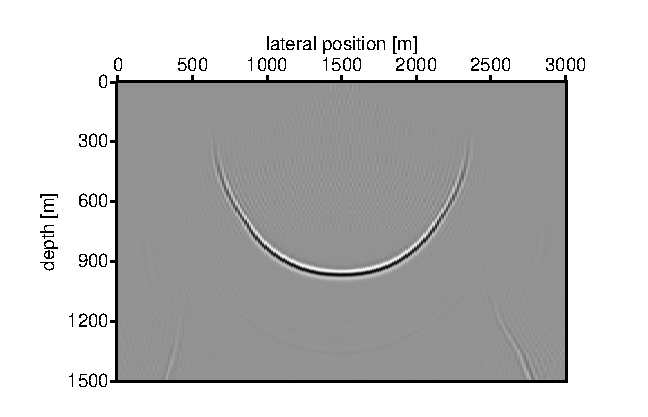
\epsfig{file=EPS/migr_puls10.eps,height=5cm}}
\end{pspicture}
\caption{ Pulse responses of the migration program for two different operators. Left show the smooth WSLQ operator and right
shows the best selected WLSQ operator.} \label{migr1}
\end{figure}
%


\subsection{To do}
3D extension is available on request.

\subsection{References}

Thorbecke, J., Wapenaar, K.,  and Swinnen, G., 2004, Design of one way wavefield extrapolation operators, using smooth functions in WLSQ optimization.: {\bf Geophysics}, pages 1037--1045.
